% Method section (draft v2, 2026-11). Self-contained: % Method section (draft v2, 2026-11). Self-contained: % Method section (draft v2, 2026-11). Self-contained: % Method section (draft v2, 2026-11). Self-contained: \input{method_section} from main.tex once approved.
% No result numbers here except dataset statistics; all performance numbers stay in Sec. 4.
\section{Method}
\label{sec:method}

\begin{figure}[t]
\centering
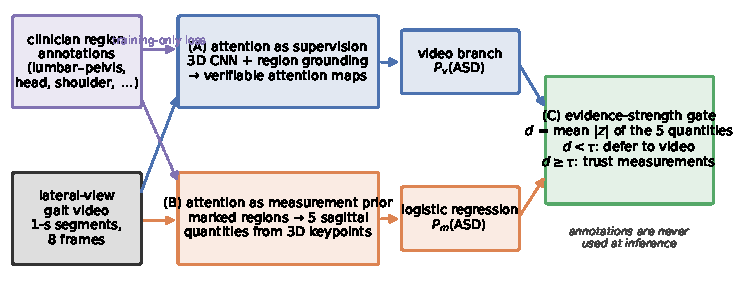
\includegraphics[width=0.86\linewidth]{figs/fig1_pipeline.pdf}
\caption{Overview. Clinician region annotations are used once, offline, to decide \emph{what to
measure} (Sec.~\ref{sec:prior}); at test time a patient needs only the video. The measurement
branch and a video branch are fused per patient by an evidence-strength gate
(Sec.~\ref{sec:gate}). The conventional use of the same annotations, as attention
supervision, serves as the contrast (Sec.~\ref{sec:sup}).}
\label{fig:pipeline}
\end{figure}

\subsection{Setting and notation}
\label{sec:setting}

\paragraph{Data.} We use lateral-view walking videos of 79 patients (54 \asd, 25 non-\asd;
the latter pools dropped-head syndrome and lumbar stenosis / hip osteoarthritis). The 1,889
videos are cut into 1-s segments of $T{=}8$ uniformly sampled frames (14,048 segments).
Patient $i$ has label $y_i\in\{0,1\}$ and a set of segments $\mathcal{S}_i$. Camera-frame 3D
keypoints from SAM-3D-Body~\cite{TODO_sam3dbody} are available for 67 patients, the primary
cohort; 2D keypoints come from YOLOv8-pose~\cite{TODO_yolov8pose}. We write $x$ for the
walking direction and $y$ for the vertical, so the $x$--$y$ plane is the sagittal plane.

\paragraph{Clinician annotation.} Two spine surgeons marked, per patient, the body regions
they attend to out of five candidates. At least one of them marked \emph{lumbar--pelvis} for
72\% of patients, \emph{head} for 47\%, \emph{shoulder} for 23\%, \emph{wrist} for 3\% and
\emph{foot} for 1\%; only six combinations occur and the two annotators agree on 45.7\% of
region decisions. We therefore treat the annotation as a \emph{group-level prior}: the set
$\mathcal{R}^{\star}=\{\text{lumbar--pelvis},\ \text{head},\ \text{shoulder}\}$ of regions that
clinicians look at, not a per-patient input.

\subsection{Contrast: attention as supervision}
\label{sec:sup}

The conventional way to use $\mathcal{R}^{\star}$ is to supervise where a network looks. Our
contrast model queries the token grid of a Kinetics-pretrained slow\_r50 with $R{=}5$ learned
concept vectors, one per region, by cross-attention; concept $r$ yields a spatio-temporal
attention map $A_r$ and a pooled feature. A presence head predicts whether region $r$ is
marked, and the classifier consumes the presence-weighted concept features together with a
global feature. Training minimises
\begin{equation}
\mathcal{L}=\mathcal{L}_{\mathrm{cls}}+\lambda_p\,\mathcal{L}_{\mathrm{presence}}
+\lambda_g\,\mathcal{L}_{\mathrm{ground}},
\label{eq:sup}
\end{equation}
where $\mathcal{L}_{\mathrm{presence}}$ is a soft cross-entropy against the two-annotator
targets $\{0,\tfrac12,1\}$ and $\mathcal{L}_{\mathrm{ground}}$ is the KL divergence between
$A_r$ and a Gaussian rendering $M_r$ of the region on the skeleton, weighted by the soft
presence. Inference uses the video only. We report the attention alignment
$\sum_n A_r(n)\,\hat M_r(n)$ with $\hat M_r=M_r/\max M_r$, for which a uniform map scores
$0.068$.

\subsection{Attention as a measurement prior}
\label{sec:prior}

Instead of telling a network where to look, we let $\mathcal{R}^{\star}$ decide which
quantities to compute. Let $\mathbf{s}_t,\mathbf{h}_t,\mathbf{e}_t$ be the midpoints of the
two shoulders, hips and ears in frame $t$, and $\mathbf{h}^{\ell}_t,\mathbf{k}^{\ell}_t$ the
hip and knee of leg $\ell\in\{\mathrm{L},\mathrm{R}\}$. With the trunk vector
$\mathbf{u}_t=\mathbf{s}_t-\mathbf{h}_t$ and the hip angle
$\phi^{\ell}_t=\angle(\mathbf{s}_t,\mathbf{h}^{\ell}_t,\mathbf{k}^{\ell}_t)$, the three
regions give five sagittal quantities per segment (Table~\ref{tab:quantities}):
\begin{align}
m_1 &= \tfrac1T\textstyle\sum_t \operatorname{atan2}\!\big(u_{t,x},\,u_{t,y}\big) && \text{(trunk lean)} \nonumber\\
m_2 &= \tfrac1T\textstyle\sum_t u_{t,x}/\lVert\mathbf{u}_t\rVert && \text{(shoulder offset)} \nonumber\\
m_3 &= \tfrac1T\textstyle\sum_t \operatorname{atan2}\!\big(e_{t,x}-s_{t,x},\,e_{t,y}-s_{t,y}\big) && \text{(head forward)} \label{eq:quantities}\\
m_4 &= 180^\circ-\min\nolimits_{t,\ell}\,\phi^{\ell}_t && \text{(maximum hip flexion)} \nonumber\\
m_5 &= \max\nolimits_{t,\ell}\,\phi^{\ell}_t-\min\nolimits_{t,\ell}\,\phi^{\ell}_t && \text{(hip range)} \nonumber
\end{align}
Angles are in degrees and positive in the walking direction. A patient is represented by the
mean over its segments, $\mathbf{m}_i=\frac{1}{|\mathcal{S}_i|}\sum_{s\in\mathcal{S}_i}\mathbf{m}_{i,s}\in\mathbb{R}^5$.

\begin{table}[t]
\centering
\caption{The five clinician-defined quantities. All are computed from 3D keypoints in the
sagittal plane over one 1-s segment and averaged over the patient's segments.}
\label{tab:quantities}
\setlength{\tabcolsep}{5pt}
\begin{tabular}{@{}llll@{}}
\toprule
Region & Quantity & Landmarks & Unit \\
\midrule
Lumbar--pelvis & trunk lean $m_1$ & shoulder mid., hip mid. & deg \\
Shoulder & shoulder offset $m_2$ & shoulder mid., hip mid. & trunk lengths \\
Head & head forward $m_3$ & ear mid., shoulder mid. & deg \\
Lumbar--pelvis & max.\ hip flexion $m_4$ & shoulder mid., hip, knee & deg \\
Lumbar--pelvis & hip range $m_5$ & shoulder mid., hip, knee & deg \\
\bottomrule
\end{tabular}
\end{table}

\paragraph{Measurement branch.} With $\boldsymbol\mu,\boldsymbol\sigma$ the mean and standard
deviation of the training patients, $\mathbf{z}_i=(\mathbf{m}_i-\boldsymbol\mu)/\boldsymbol\sigma$
is classified by a class-balanced logistic regression,
\begin{equation}
P^{m}_i=\sigma\!\big(\boldsymbol\beta^{\top}\mathbf{z}_i+\beta_0\big),
\label{eq:lr}
\end{equation}
with the default regularisation ($C{=}1$). The model has six parameters and nothing is tuned
on the outcome.

\paragraph{Deriving the quantities with a language model.}
% ---- optional subsection: keep only if the LLM experiment goes into the paper ----
The step from $\mathcal{R}^{\star}$ to Eq.~\eqref{eq:quantities} is a design choice. To make
it reproducible we also let a language model make it. The model receives (i) the region names
in $\mathcal{R}^{\star}$, (ii) the list of available landmarks and (iii) a measurement
grammar $\mathcal{G}$: a two-landmark quantity (sagittal inclination, anterior offset, height
or lateral distance) or one of eight joint angles, each summarised over a segment by its
mean, extreme or range. It returns $K{=}5$ measurements in $\mathcal{G}$, which are then
computed geometrically exactly as above. The model sees no video, no keypoint value and no
label; neither the disease nor any specific measurement is named in the prompt. We sample it
$N$ times and, as controls, replace $\mathcal{R}^{\star}$ by three regions that clinicians
rarely mark (knees, feet/ankles, wrists/elbows) or omit the regions.

\paragraph{Is it the selection?} To test whether the choice of quantities matters we build a
\emph{bank} of 1,272 candidates in the same grammar (all pairwise landmark quantities and
twelve chain angles, as segment means, extremes and ranges), each tagged with the regions it
touches. We compare the five quantities with random draws from the bank, with quantities
restricted to unmarked regions, and with data-driven selection over the whole bank
($\ell_1$ logistic regression, random forests, gradient boosting).

\subsection{Video branch}
\label{sec:video}

The video branch is a slow\_r50~\cite{TODO_slowfast} pretrained on Kinetics-400 and fine-tuned
on the segments with cross-entropy. Its patient-level probability is the mean over segments,
$P^{v}_i=\frac{1}{|\mathcal{S}_i|}\sum_{s\in\mathcal{S}_i}p^{v}_{i,s}$. Any segment classifier can
take this role; we also report a video transformer and the region-grounded model of
Sec.~\ref{sec:sup}.

\subsection{Evidence-strength gating}
\label{sec:gate}

The two branches fail on different patients. A measurement vector close to the population
norm says little about the diagnosis, whereas a strongly deviating one is decisive. We
quantify this by the \emph{deviation}
\begin{equation}
d_i=\frac{1}{5\,|\mathcal{S}_i|}\sum_{s\in\mathcal{S}_i}\sum_{j=1}^{5}
\left|\frac{m_{i,s,j}-\mu^{\mathrm{seg}}_j}{\sigma^{\mathrm{seg}}_j}\right| ,
\label{eq:dev}
\end{equation}
the patient's mean absolute $z$-score, with segment-level statistics
$\mu^{\mathrm{seg}},\sigma^{\mathrm{seg}}$ taken from the training patients only. The fused
probability is
\begin{equation}
P_i=w_i\,P^{m}_i+(1-w_i)\,P^{v}_i,\qquad
w_i=\begin{cases} w_{\mathrm{lo}} & d_i<\tau\\ w_{\mathrm{hi}} & d_i\ge\tau\end{cases},
\label{eq:gate}
\end{equation}
where the threshold $\tau=Q_q(\{d_k\}_{k\in\mathrm{train}})$ is the $q$-quantile of the deviations of the training patients. Patients whose measurements are unremarkable are deferred to
the video branch; the others are decided by the measurements. The rule has three parameters
$(q,w_{\mathrm{lo}},w_{\mathrm{hi}})$, selected on the training patients of each outer fold
(Algorithm~\ref{alg:gate}); the test fold only applies it. It is readable: for every patient
it reports the five values, their deviation, and which branch decided.

\begin{algorithm}[t]
\caption{Evidence-strength gate, nested in $F$ patient folds}
\label{alg:gate}
\begin{algorithmic}[1]
\Require out-of-fold probabilities $P^{m}_i,P^{v}_i$, segment measurements $\mathbf{m}_{i,s}$, labels $y_i$
\For{each outer fold $f=1,\dots,F$ with training patients $\mathcal{T}_f$ and test patients $\mathcal{V}_f$}
  \State compute $\mu^{\mathrm{seg}},\sigma^{\mathrm{seg}}$ on $\mathcal{T}_f$ and $d_i$ for all $i$ by Eq.~\eqref{eq:dev}
  \For{$(q,w_{\mathrm{lo}},w_{\mathrm{hi}})\in\{0.2,0.25,\dots,0.5\}\times\{0,0.25,0.5\}\times\{0.75,1\}$}
     \State $\tau\gets Q_q(\{d_k\}_{k\in\mathcal{T}_f})$; fuse $\mathcal{T}_f$ by Eq.~\eqref{eq:gate}
     \State score by balanced accuracy on $\mathcal{T}_f$ (ties: lower negative log-likelihood)
  \EndFor
  \State apply the best $(\tau,w_{\mathrm{lo}},w_{\mathrm{hi}})$ to $\mathcal{V}_f$
\EndFor
\State \Return fused probabilities $P_i$ for all patients
\end{algorithmic}
\end{algorithm}

\paragraph{Fusion baselines.} Under the same nested protocol we compare a fixed $w{=}0.5$, a
global $w$ selected on the training patients, stacking (logistic regression on the two
logits), and a learnable sigmoid gate $w_i=\sigma(\boldsymbol\theta^{\top}\mathbf{r}_i)$ on six
reliability features $\mathbf{r}_i$ (video confidence and segment disagreement, number of
segments, measurement confidence, fraction of segments without 3D, and $d_i$), fitted by
class-balanced likelihood with an inner-selected $\ell_2$ penalty. As a control for
Eq.~\eqref{eq:gate} we permute $d_i$ across patients.
 from main.tex once approved.
% No result numbers here except dataset statistics; all performance numbers stay in Sec. 4.
\section{Method}
\label{sec:method}

\begin{figure}[t]
\centering
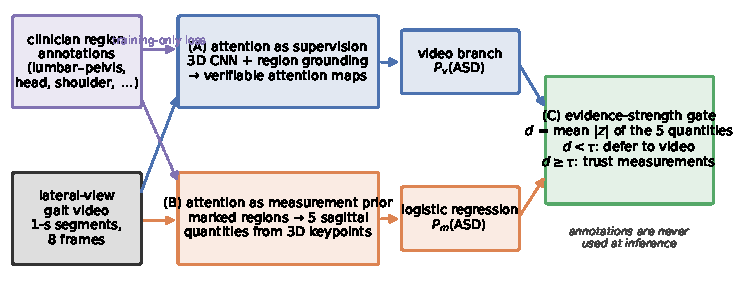
\includegraphics[width=0.86\linewidth]{figs/fig1_pipeline.pdf}
\caption{Overview. Clinician region annotations are used once, offline, to decide \emph{what to
measure} (Sec.~\ref{sec:prior}); at test time a patient needs only the video. The measurement
branch and a video branch are fused per patient by an evidence-strength gate
(Sec.~\ref{sec:gate}). The conventional use of the same annotations, as attention
supervision, serves as the contrast (Sec.~\ref{sec:sup}).}
\label{fig:pipeline}
\end{figure}

\subsection{Setting and notation}
\label{sec:setting}

\paragraph{Data.} We use lateral-view walking videos of 79 patients (54 \asd, 25 non-\asd;
the latter pools dropped-head syndrome and lumbar stenosis / hip osteoarthritis). The 1,889
videos are cut into 1-s segments of $T{=}8$ uniformly sampled frames (14,048 segments).
Patient $i$ has label $y_i\in\{0,1\}$ and a set of segments $\mathcal{S}_i$. Camera-frame 3D
keypoints from SAM-3D-Body~\cite{TODO_sam3dbody} are available for 67 patients, the primary
cohort; 2D keypoints come from YOLOv8-pose~\cite{TODO_yolov8pose}. We write $x$ for the
walking direction and $y$ for the vertical, so the $x$--$y$ plane is the sagittal plane.

\paragraph{Clinician annotation.} Two spine surgeons marked, per patient, the body regions
they attend to out of five candidates. At least one of them marked \emph{lumbar--pelvis} for
72\% of patients, \emph{head} for 47\%, \emph{shoulder} for 23\%, \emph{wrist} for 3\% and
\emph{foot} for 1\%; only six combinations occur and the two annotators agree on 45.7\% of
region decisions. We therefore treat the annotation as a \emph{group-level prior}: the set
$\mathcal{R}^{\star}=\{\text{lumbar--pelvis},\ \text{head},\ \text{shoulder}\}$ of regions that
clinicians look at, not a per-patient input.

\subsection{Contrast: attention as supervision}
\label{sec:sup}

The conventional way to use $\mathcal{R}^{\star}$ is to supervise where a network looks. Our
contrast model queries the token grid of a Kinetics-pretrained slow\_r50 with $R{=}5$ learned
concept vectors, one per region, by cross-attention; concept $r$ yields a spatio-temporal
attention map $A_r$ and a pooled feature. A presence head predicts whether region $r$ is
marked, and the classifier consumes the presence-weighted concept features together with a
global feature. Training minimises
\begin{equation}
\mathcal{L}=\mathcal{L}_{\mathrm{cls}}+\lambda_p\,\mathcal{L}_{\mathrm{presence}}
+\lambda_g\,\mathcal{L}_{\mathrm{ground}},
\label{eq:sup}
\end{equation}
where $\mathcal{L}_{\mathrm{presence}}$ is a soft cross-entropy against the two-annotator
targets $\{0,\tfrac12,1\}$ and $\mathcal{L}_{\mathrm{ground}}$ is the KL divergence between
$A_r$ and a Gaussian rendering $M_r$ of the region on the skeleton, weighted by the soft
presence. Inference uses the video only. We report the attention alignment
$\sum_n A_r(n)\,\hat M_r(n)$ with $\hat M_r=M_r/\max M_r$, for which a uniform map scores
$0.068$.

\subsection{Attention as a measurement prior}
\label{sec:prior}

Instead of telling a network where to look, we let $\mathcal{R}^{\star}$ decide which
quantities to compute. Let $\mathbf{s}_t,\mathbf{h}_t,\mathbf{e}_t$ be the midpoints of the
two shoulders, hips and ears in frame $t$, and $\mathbf{h}^{\ell}_t,\mathbf{k}^{\ell}_t$ the
hip and knee of leg $\ell\in\{\mathrm{L},\mathrm{R}\}$. With the trunk vector
$\mathbf{u}_t=\mathbf{s}_t-\mathbf{h}_t$ and the hip angle
$\phi^{\ell}_t=\angle(\mathbf{s}_t,\mathbf{h}^{\ell}_t,\mathbf{k}^{\ell}_t)$, the three
regions give five sagittal quantities per segment (Table~\ref{tab:quantities}):
\begin{align}
m_1 &= \tfrac1T\textstyle\sum_t \operatorname{atan2}\!\big(u_{t,x},\,u_{t,y}\big) && \text{(trunk lean)} \nonumber\\
m_2 &= \tfrac1T\textstyle\sum_t u_{t,x}/\lVert\mathbf{u}_t\rVert && \text{(shoulder offset)} \nonumber\\
m_3 &= \tfrac1T\textstyle\sum_t \operatorname{atan2}\!\big(e_{t,x}-s_{t,x},\,e_{t,y}-s_{t,y}\big) && \text{(head forward)} \label{eq:quantities}\\
m_4 &= 180^\circ-\min\nolimits_{t,\ell}\,\phi^{\ell}_t && \text{(maximum hip flexion)} \nonumber\\
m_5 &= \max\nolimits_{t,\ell}\,\phi^{\ell}_t-\min\nolimits_{t,\ell}\,\phi^{\ell}_t && \text{(hip range)} \nonumber
\end{align}
Angles are in degrees and positive in the walking direction. A patient is represented by the
mean over its segments, $\mathbf{m}_i=\frac{1}{|\mathcal{S}_i|}\sum_{s\in\mathcal{S}_i}\mathbf{m}_{i,s}\in\mathbb{R}^5$.

\begin{table}[t]
\centering
\caption{The five clinician-defined quantities. All are computed from 3D keypoints in the
sagittal plane over one 1-s segment and averaged over the patient's segments.}
\label{tab:quantities}
\setlength{\tabcolsep}{5pt}
\begin{tabular}{@{}llll@{}}
\toprule
Region & Quantity & Landmarks & Unit \\
\midrule
Lumbar--pelvis & trunk lean $m_1$ & shoulder mid., hip mid. & deg \\
Shoulder & shoulder offset $m_2$ & shoulder mid., hip mid. & trunk lengths \\
Head & head forward $m_3$ & ear mid., shoulder mid. & deg \\
Lumbar--pelvis & max.\ hip flexion $m_4$ & shoulder mid., hip, knee & deg \\
Lumbar--pelvis & hip range $m_5$ & shoulder mid., hip, knee & deg \\
\bottomrule
\end{tabular}
\end{table}

\paragraph{Measurement branch.} With $\boldsymbol\mu,\boldsymbol\sigma$ the mean and standard
deviation of the training patients, $\mathbf{z}_i=(\mathbf{m}_i-\boldsymbol\mu)/\boldsymbol\sigma$
is classified by a class-balanced logistic regression,
\begin{equation}
P^{m}_i=\sigma\!\big(\boldsymbol\beta^{\top}\mathbf{z}_i+\beta_0\big),
\label{eq:lr}
\end{equation}
with the default regularisation ($C{=}1$). The model has six parameters and nothing is tuned
on the outcome.

\paragraph{Deriving the quantities with a language model.}
% ---- optional subsection: keep only if the LLM experiment goes into the paper ----
The step from $\mathcal{R}^{\star}$ to Eq.~\eqref{eq:quantities} is a design choice. To make
it reproducible we also let a language model make it. The model receives (i) the region names
in $\mathcal{R}^{\star}$, (ii) the list of available landmarks and (iii) a measurement
grammar $\mathcal{G}$: a two-landmark quantity (sagittal inclination, anterior offset, height
or lateral distance) or one of eight joint angles, each summarised over a segment by its
mean, extreme or range. It returns $K{=}5$ measurements in $\mathcal{G}$, which are then
computed geometrically exactly as above. The model sees no video, no keypoint value and no
label; neither the disease nor any specific measurement is named in the prompt. We sample it
$N$ times and, as controls, replace $\mathcal{R}^{\star}$ by three regions that clinicians
rarely mark (knees, feet/ankles, wrists/elbows) or omit the regions.

\paragraph{Is it the selection?} To test whether the choice of quantities matters we build a
\emph{bank} of 1,272 candidates in the same grammar (all pairwise landmark quantities and
twelve chain angles, as segment means, extremes and ranges), each tagged with the regions it
touches. We compare the five quantities with random draws from the bank, with quantities
restricted to unmarked regions, and with data-driven selection over the whole bank
($\ell_1$ logistic regression, random forests, gradient boosting).

\subsection{Video branch}
\label{sec:video}

The video branch is a slow\_r50~\cite{TODO_slowfast} pretrained on Kinetics-400 and fine-tuned
on the segments with cross-entropy. Its patient-level probability is the mean over segments,
$P^{v}_i=\frac{1}{|\mathcal{S}_i|}\sum_{s\in\mathcal{S}_i}p^{v}_{i,s}$. Any segment classifier can
take this role; we also report a video transformer and the region-grounded model of
Sec.~\ref{sec:sup}.

\subsection{Evidence-strength gating}
\label{sec:gate}

The two branches fail on different patients. A measurement vector close to the population
norm says little about the diagnosis, whereas a strongly deviating one is decisive. We
quantify this by the \emph{deviation}
\begin{equation}
d_i=\frac{1}{5\,|\mathcal{S}_i|}\sum_{s\in\mathcal{S}_i}\sum_{j=1}^{5}
\left|\frac{m_{i,s,j}-\mu^{\mathrm{seg}}_j}{\sigma^{\mathrm{seg}}_j}\right| ,
\label{eq:dev}
\end{equation}
the patient's mean absolute $z$-score, with segment-level statistics
$\mu^{\mathrm{seg}},\sigma^{\mathrm{seg}}$ taken from the training patients only. The fused
probability is
\begin{equation}
P_i=w_i\,P^{m}_i+(1-w_i)\,P^{v}_i,\qquad
w_i=\begin{cases} w_{\mathrm{lo}} & d_i<\tau\\ w_{\mathrm{hi}} & d_i\ge\tau\end{cases},
\label{eq:gate}
\end{equation}
where the threshold $\tau=Q_q(\{d_k\}_{k\in\mathrm{train}})$ is the $q$-quantile of the deviations of the training patients. Patients whose measurements are unremarkable are deferred to
the video branch; the others are decided by the measurements. The rule has three parameters
$(q,w_{\mathrm{lo}},w_{\mathrm{hi}})$, selected on the training patients of each outer fold
(Algorithm~\ref{alg:gate}); the test fold only applies it. It is readable: for every patient
it reports the five values, their deviation, and which branch decided.

\begin{algorithm}[t]
\caption{Evidence-strength gate, nested in $F$ patient folds}
\label{alg:gate}
\begin{algorithmic}[1]
\Require out-of-fold probabilities $P^{m}_i,P^{v}_i$, segment measurements $\mathbf{m}_{i,s}$, labels $y_i$
\For{each outer fold $f=1,\dots,F$ with training patients $\mathcal{T}_f$ and test patients $\mathcal{V}_f$}
  \State compute $\mu^{\mathrm{seg}},\sigma^{\mathrm{seg}}$ on $\mathcal{T}_f$ and $d_i$ for all $i$ by Eq.~\eqref{eq:dev}
  \For{$(q,w_{\mathrm{lo}},w_{\mathrm{hi}})\in\{0.2,0.25,\dots,0.5\}\times\{0,0.25,0.5\}\times\{0.75,1\}$}
     \State $\tau\gets Q_q(\{d_k\}_{k\in\mathcal{T}_f})$; fuse $\mathcal{T}_f$ by Eq.~\eqref{eq:gate}
     \State score by balanced accuracy on $\mathcal{T}_f$ (ties: lower negative log-likelihood)
  \EndFor
  \State apply the best $(\tau,w_{\mathrm{lo}},w_{\mathrm{hi}})$ to $\mathcal{V}_f$
\EndFor
\State \Return fused probabilities $P_i$ for all patients
\end{algorithmic}
\end{algorithm}

\paragraph{Fusion baselines.} Under the same nested protocol we compare a fixed $w{=}0.5$, a
global $w$ selected on the training patients, stacking (logistic regression on the two
logits), and a learnable sigmoid gate $w_i=\sigma(\boldsymbol\theta^{\top}\mathbf{r}_i)$ on six
reliability features $\mathbf{r}_i$ (video confidence and segment disagreement, number of
segments, measurement confidence, fraction of segments without 3D, and $d_i$), fitted by
class-balanced likelihood with an inner-selected $\ell_2$ penalty. As a control for
Eq.~\eqref{eq:gate} we permute $d_i$ across patients.
 from main.tex once approved.
% No result numbers here except dataset statistics; all performance numbers stay in Sec. 4.
\section{Method}
\label{sec:method}

\begin{figure}[t]
\centering
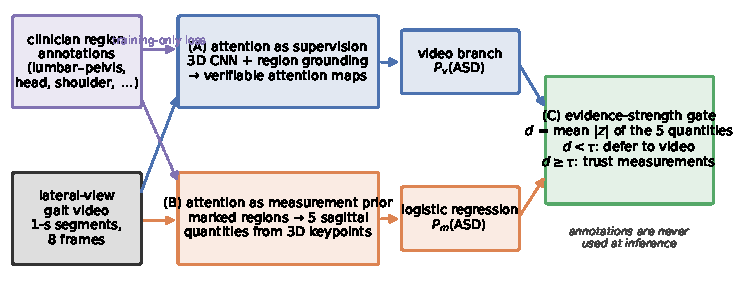
\includegraphics[width=0.86\linewidth]{figs/fig1_pipeline.pdf}
\caption{Overview. Clinician region annotations are used once, offline, to decide \emph{what to
measure} (Sec.~\ref{sec:prior}); at test time a patient needs only the video. The measurement
branch and a video branch are fused per patient by an evidence-strength gate
(Sec.~\ref{sec:gate}). The conventional use of the same annotations, as attention
supervision, serves as the contrast (Sec.~\ref{sec:sup}).}
\label{fig:pipeline}
\end{figure}

\subsection{Setting and notation}
\label{sec:setting}

\paragraph{Data.} We use lateral-view walking videos of 79 patients (54 \asd, 25 non-\asd;
the latter pools dropped-head syndrome and lumbar stenosis / hip osteoarthritis). The 1,889
videos are cut into 1-s segments of $T{=}8$ uniformly sampled frames (14,048 segments).
Patient $i$ has label $y_i\in\{0,1\}$ and a set of segments $\mathcal{S}_i$. Camera-frame 3D
keypoints from SAM-3D-Body~\cite{TODO_sam3dbody} are available for 67 patients, the primary
cohort; 2D keypoints come from YOLOv8-pose~\cite{TODO_yolov8pose}. We write $x$ for the
walking direction and $y$ for the vertical, so the $x$--$y$ plane is the sagittal plane.

\paragraph{Clinician annotation.} Two spine surgeons marked, per patient, the body regions
they attend to out of five candidates. At least one of them marked \emph{lumbar--pelvis} for
72\% of patients, \emph{head} for 47\%, \emph{shoulder} for 23\%, \emph{wrist} for 3\% and
\emph{foot} for 1\%; only six combinations occur and the two annotators agree on 45.7\% of
region decisions. We therefore treat the annotation as a \emph{group-level prior}: the set
$\mathcal{R}^{\star}=\{\text{lumbar--pelvis},\ \text{head},\ \text{shoulder}\}$ of regions that
clinicians look at, not a per-patient input.

\subsection{Contrast: attention as supervision}
\label{sec:sup}

The conventional way to use $\mathcal{R}^{\star}$ is to supervise where a network looks. Our
contrast model queries the token grid of a Kinetics-pretrained slow\_r50 with $R{=}5$ learned
concept vectors, one per region, by cross-attention; concept $r$ yields a spatio-temporal
attention map $A_r$ and a pooled feature. A presence head predicts whether region $r$ is
marked, and the classifier consumes the presence-weighted concept features together with a
global feature. Training minimises
\begin{equation}
\mathcal{L}=\mathcal{L}_{\mathrm{cls}}+\lambda_p\,\mathcal{L}_{\mathrm{presence}}
+\lambda_g\,\mathcal{L}_{\mathrm{ground}},
\label{eq:sup}
\end{equation}
where $\mathcal{L}_{\mathrm{presence}}$ is a soft cross-entropy against the two-annotator
targets $\{0,\tfrac12,1\}$ and $\mathcal{L}_{\mathrm{ground}}$ is the KL divergence between
$A_r$ and a Gaussian rendering $M_r$ of the region on the skeleton, weighted by the soft
presence. Inference uses the video only. We report the attention alignment
$\sum_n A_r(n)\,\hat M_r(n)$ with $\hat M_r=M_r/\max M_r$, for which a uniform map scores
$0.068$.

\subsection{Attention as a measurement prior}
\label{sec:prior}

Instead of telling a network where to look, we let $\mathcal{R}^{\star}$ decide which
quantities to compute. Let $\mathbf{s}_t,\mathbf{h}_t,\mathbf{e}_t$ be the midpoints of the
two shoulders, hips and ears in frame $t$, and $\mathbf{h}^{\ell}_t,\mathbf{k}^{\ell}_t$ the
hip and knee of leg $\ell\in\{\mathrm{L},\mathrm{R}\}$. With the trunk vector
$\mathbf{u}_t=\mathbf{s}_t-\mathbf{h}_t$ and the hip angle
$\phi^{\ell}_t=\angle(\mathbf{s}_t,\mathbf{h}^{\ell}_t,\mathbf{k}^{\ell}_t)$, the three
regions give five sagittal quantities per segment (Table~\ref{tab:quantities}):
\begin{align}
m_1 &= \tfrac1T\textstyle\sum_t \operatorname{atan2}\!\big(u_{t,x},\,u_{t,y}\big) && \text{(trunk lean)} \nonumber\\
m_2 &= \tfrac1T\textstyle\sum_t u_{t,x}/\lVert\mathbf{u}_t\rVert && \text{(shoulder offset)} \nonumber\\
m_3 &= \tfrac1T\textstyle\sum_t \operatorname{atan2}\!\big(e_{t,x}-s_{t,x},\,e_{t,y}-s_{t,y}\big) && \text{(head forward)} \label{eq:quantities}\\
m_4 &= 180^\circ-\min\nolimits_{t,\ell}\,\phi^{\ell}_t && \text{(maximum hip flexion)} \nonumber\\
m_5 &= \max\nolimits_{t,\ell}\,\phi^{\ell}_t-\min\nolimits_{t,\ell}\,\phi^{\ell}_t && \text{(hip range)} \nonumber
\end{align}
Angles are in degrees and positive in the walking direction. A patient is represented by the
mean over its segments, $\mathbf{m}_i=\frac{1}{|\mathcal{S}_i|}\sum_{s\in\mathcal{S}_i}\mathbf{m}_{i,s}\in\mathbb{R}^5$.

\begin{table}[t]
\centering
\caption{The five clinician-defined quantities. All are computed from 3D keypoints in the
sagittal plane over one 1-s segment and averaged over the patient's segments.}
\label{tab:quantities}
\setlength{\tabcolsep}{5pt}
\begin{tabular}{@{}llll@{}}
\toprule
Region & Quantity & Landmarks & Unit \\
\midrule
Lumbar--pelvis & trunk lean $m_1$ & shoulder mid., hip mid. & deg \\
Shoulder & shoulder offset $m_2$ & shoulder mid., hip mid. & trunk lengths \\
Head & head forward $m_3$ & ear mid., shoulder mid. & deg \\
Lumbar--pelvis & max.\ hip flexion $m_4$ & shoulder mid., hip, knee & deg \\
Lumbar--pelvis & hip range $m_5$ & shoulder mid., hip, knee & deg \\
\bottomrule
\end{tabular}
\end{table}

\paragraph{Measurement branch.} With $\boldsymbol\mu,\boldsymbol\sigma$ the mean and standard
deviation of the training patients, $\mathbf{z}_i=(\mathbf{m}_i-\boldsymbol\mu)/\boldsymbol\sigma$
is classified by a class-balanced logistic regression,
\begin{equation}
P^{m}_i=\sigma\!\big(\boldsymbol\beta^{\top}\mathbf{z}_i+\beta_0\big),
\label{eq:lr}
\end{equation}
with the default regularisation ($C{=}1$). The model has six parameters and nothing is tuned
on the outcome.

\paragraph{Deriving the quantities with a language model.}
% ---- optional subsection: keep only if the LLM experiment goes into the paper ----
The step from $\mathcal{R}^{\star}$ to Eq.~\eqref{eq:quantities} is a design choice. To make
it reproducible we also let a language model make it. The model receives (i) the region names
in $\mathcal{R}^{\star}$, (ii) the list of available landmarks and (iii) a measurement
grammar $\mathcal{G}$: a two-landmark quantity (sagittal inclination, anterior offset, height
or lateral distance) or one of eight joint angles, each summarised over a segment by its
mean, extreme or range. It returns $K{=}5$ measurements in $\mathcal{G}$, which are then
computed geometrically exactly as above. The model sees no video, no keypoint value and no
label; neither the disease nor any specific measurement is named in the prompt. We sample it
$N$ times and, as controls, replace $\mathcal{R}^{\star}$ by three regions that clinicians
rarely mark (knees, feet/ankles, wrists/elbows) or omit the regions.

\paragraph{Is it the selection?} To test whether the choice of quantities matters we build a
\emph{bank} of 1,272 candidates in the same grammar (all pairwise landmark quantities and
twelve chain angles, as segment means, extremes and ranges), each tagged with the regions it
touches. We compare the five quantities with random draws from the bank, with quantities
restricted to unmarked regions, and with data-driven selection over the whole bank
($\ell_1$ logistic regression, random forests, gradient boosting).

\subsection{Video branch}
\label{sec:video}

The video branch is a slow\_r50~\cite{TODO_slowfast} pretrained on Kinetics-400 and fine-tuned
on the segments with cross-entropy. Its patient-level probability is the mean over segments,
$P^{v}_i=\frac{1}{|\mathcal{S}_i|}\sum_{s\in\mathcal{S}_i}p^{v}_{i,s}$. Any segment classifier can
take this role; we also report a video transformer and the region-grounded model of
Sec.~\ref{sec:sup}.

\subsection{Evidence-strength gating}
\label{sec:gate}

The two branches fail on different patients. A measurement vector close to the population
norm says little about the diagnosis, whereas a strongly deviating one is decisive. We
quantify this by the \emph{deviation}
\begin{equation}
d_i=\frac{1}{5\,|\mathcal{S}_i|}\sum_{s\in\mathcal{S}_i}\sum_{j=1}^{5}
\left|\frac{m_{i,s,j}-\mu^{\mathrm{seg}}_j}{\sigma^{\mathrm{seg}}_j}\right| ,
\label{eq:dev}
\end{equation}
the patient's mean absolute $z$-score, with segment-level statistics
$\mu^{\mathrm{seg}},\sigma^{\mathrm{seg}}$ taken from the training patients only. The fused
probability is
\begin{equation}
P_i=w_i\,P^{m}_i+(1-w_i)\,P^{v}_i,\qquad
w_i=\begin{cases} w_{\mathrm{lo}} & d_i<\tau\\ w_{\mathrm{hi}} & d_i\ge\tau\end{cases},
\label{eq:gate}
\end{equation}
where the threshold $\tau=Q_q(\{d_k\}_{k\in\mathrm{train}})$ is the $q$-quantile of the deviations of the training patients. Patients whose measurements are unremarkable are deferred to
the video branch; the others are decided by the measurements. The rule has three parameters
$(q,w_{\mathrm{lo}},w_{\mathrm{hi}})$, selected on the training patients of each outer fold
(Algorithm~\ref{alg:gate}); the test fold only applies it. It is readable: for every patient
it reports the five values, their deviation, and which branch decided.

\begin{algorithm}[t]
\caption{Evidence-strength gate, nested in $F$ patient folds}
\label{alg:gate}
\begin{algorithmic}[1]
\Require out-of-fold probabilities $P^{m}_i,P^{v}_i$, segment measurements $\mathbf{m}_{i,s}$, labels $y_i$
\For{each outer fold $f=1,\dots,F$ with training patients $\mathcal{T}_f$ and test patients $\mathcal{V}_f$}
  \State compute $\mu^{\mathrm{seg}},\sigma^{\mathrm{seg}}$ on $\mathcal{T}_f$ and $d_i$ for all $i$ by Eq.~\eqref{eq:dev}
  \For{$(q,w_{\mathrm{lo}},w_{\mathrm{hi}})\in\{0.2,0.25,\dots,0.5\}\times\{0,0.25,0.5\}\times\{0.75,1\}$}
     \State $\tau\gets Q_q(\{d_k\}_{k\in\mathcal{T}_f})$; fuse $\mathcal{T}_f$ by Eq.~\eqref{eq:gate}
     \State score by balanced accuracy on $\mathcal{T}_f$ (ties: lower negative log-likelihood)
  \EndFor
  \State apply the best $(\tau,w_{\mathrm{lo}},w_{\mathrm{hi}})$ to $\mathcal{V}_f$
\EndFor
\State \Return fused probabilities $P_i$ for all patients
\end{algorithmic}
\end{algorithm}

\paragraph{Fusion baselines.} Under the same nested protocol we compare a fixed $w{=}0.5$, a
global $w$ selected on the training patients, stacking (logistic regression on the two
logits), and a learnable sigmoid gate $w_i=\sigma(\boldsymbol\theta^{\top}\mathbf{r}_i)$ on six
reliability features $\mathbf{r}_i$ (video confidence and segment disagreement, number of
segments, measurement confidence, fraction of segments without 3D, and $d_i$), fitted by
class-balanced likelihood with an inner-selected $\ell_2$ penalty. As a control for
Eq.~\eqref{eq:gate} we permute $d_i$ across patients.
 from main.tex once approved.
% No result numbers here except dataset statistics; all performance numbers stay in Sec. 4.
\section{Method}
\label{sec:method}

\begin{figure}[t]
\centering
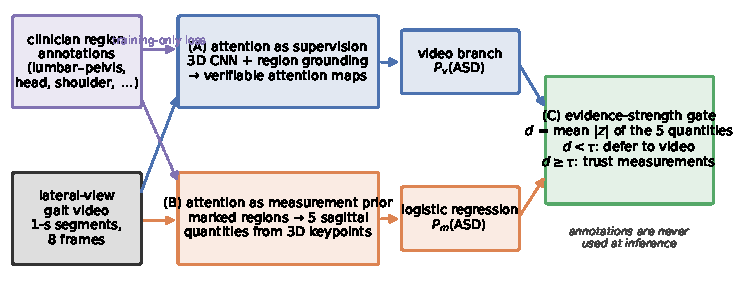
\includegraphics[width=0.86\linewidth]{figs/fig1_pipeline.pdf}
\caption{Overview. Clinician region annotations are used once, offline, to decide \emph{what to
measure} (Sec.~\ref{sec:prior}); at test time a patient needs only the video. The measurement
branch and a video branch are fused per patient by an evidence-strength gate
(Sec.~\ref{sec:gate}). The conventional use of the same annotations, as attention
supervision, serves as the contrast (Sec.~\ref{sec:sup}).}
\label{fig:pipeline}
\end{figure}

\subsection{Setting and notation}
\label{sec:setting}

\paragraph{Data.} We use lateral-view walking videos of 79 patients (54 \asd, 25 non-\asd;
the latter pools dropped-head syndrome and lumbar stenosis / hip osteoarthritis). The 1,889
videos are cut into 1-s segments of $T{=}8$ uniformly sampled frames (14,048 segments).
Patient $i$ has label $y_i\in\{0,1\}$ and a set of segments $\mathcal{S}_i$. Camera-frame 3D
keypoints from SAM-3D-Body~\cite{TODO_sam3dbody} are available for 67 patients, the primary
cohort; 2D keypoints come from YOLOv8-pose~\cite{TODO_yolov8pose}. We write $x$ for the
walking direction and $y$ for the vertical, so the $x$--$y$ plane is the sagittal plane.

\paragraph{Clinician annotation.} Two spine surgeons marked, per patient, the body regions
they attend to out of five candidates. At least one of them marked \emph{lumbar--pelvis} for
72\% of patients, \emph{head} for 47\%, \emph{shoulder} for 23\%, \emph{wrist} for 3\% and
\emph{foot} for 1\%; only six combinations occur and the two annotators agree on 45.7\% of
region decisions. We therefore treat the annotation as a \emph{group-level prior}: the set
$\mathcal{R}^{\star}=\{\text{lumbar--pelvis},\ \text{head},\ \text{shoulder}\}$ of regions that
clinicians look at, not a per-patient input.

\subsection{Contrast: attention as supervision}
\label{sec:sup}

The conventional way to use $\mathcal{R}^{\star}$ is to supervise where a network looks. Our
contrast model queries the token grid of a Kinetics-pretrained slow\_r50 with $R{=}5$ learned
concept vectors, one per region, by cross-attention; concept $r$ yields a spatio-temporal
attention map $A_r$ and a pooled feature. A presence head predicts whether region $r$ is
marked, and the classifier consumes the presence-weighted concept features together with a
global feature. Training minimises
\begin{equation}
\mathcal{L}=\mathcal{L}_{\mathrm{cls}}+\lambda_p\,\mathcal{L}_{\mathrm{presence}}
+\lambda_g\,\mathcal{L}_{\mathrm{ground}},
\label{eq:sup}
\end{equation}
where $\mathcal{L}_{\mathrm{presence}}$ is a soft cross-entropy against the two-annotator
targets $\{0,\tfrac12,1\}$ and $\mathcal{L}_{\mathrm{ground}}$ is the KL divergence between
$A_r$ and a Gaussian rendering $M_r$ of the region on the skeleton, weighted by the soft
presence. Inference uses the video only. We report the attention alignment
$\sum_n A_r(n)\,\hat M_r(n)$ with $\hat M_r=M_r/\max M_r$, for which a uniform map scores
$0.068$.

\subsection{Attention as a measurement prior}
\label{sec:prior}

Instead of telling a network where to look, we let $\mathcal{R}^{\star}$ decide which
quantities to compute. Let $\mathbf{s}_t,\mathbf{h}_t,\mathbf{e}_t$ be the midpoints of the
two shoulders, hips and ears in frame $t$, and $\mathbf{h}^{\ell}_t,\mathbf{k}^{\ell}_t$ the
hip and knee of leg $\ell\in\{\mathrm{L},\mathrm{R}\}$. With the trunk vector
$\mathbf{u}_t=\mathbf{s}_t-\mathbf{h}_t$ and the hip angle
$\phi^{\ell}_t=\angle(\mathbf{s}_t,\mathbf{h}^{\ell}_t,\mathbf{k}^{\ell}_t)$, the three
regions give five sagittal quantities per segment (Table~\ref{tab:quantities}):
\begin{align}
m_1 &= \tfrac1T\textstyle\sum_t \operatorname{atan2}\!\big(u_{t,x},\,u_{t,y}\big) && \text{(trunk lean)} \nonumber\\
m_2 &= \tfrac1T\textstyle\sum_t u_{t,x}/\lVert\mathbf{u}_t\rVert && \text{(shoulder offset)} \nonumber\\
m_3 &= \tfrac1T\textstyle\sum_t \operatorname{atan2}\!\big(e_{t,x}-s_{t,x},\,e_{t,y}-s_{t,y}\big) && \text{(head forward)} \label{eq:quantities}\\
m_4 &= 180^\circ-\min\nolimits_{t,\ell}\,\phi^{\ell}_t && \text{(maximum hip flexion)} \nonumber\\
m_5 &= \max\nolimits_{t,\ell}\,\phi^{\ell}_t-\min\nolimits_{t,\ell}\,\phi^{\ell}_t && \text{(hip range)} \nonumber
\end{align}
Angles are in degrees and positive in the walking direction. A patient is represented by the
mean over its segments, $\mathbf{m}_i=\frac{1}{|\mathcal{S}_i|}\sum_{s\in\mathcal{S}_i}\mathbf{m}_{i,s}\in\mathbb{R}^5$.

\begin{table}[t]
\centering
\caption{The five clinician-defined quantities. All are computed from 3D keypoints in the
sagittal plane over one 1-s segment and averaged over the patient's segments.}
\label{tab:quantities}
\setlength{\tabcolsep}{5pt}
\begin{tabular}{@{}llll@{}}
\toprule
Region & Quantity & Landmarks & Unit \\
\midrule
Lumbar--pelvis & trunk lean $m_1$ & shoulder mid., hip mid. & deg \\
Shoulder & shoulder offset $m_2$ & shoulder mid., hip mid. & trunk lengths \\
Head & head forward $m_3$ & ear mid., shoulder mid. & deg \\
Lumbar--pelvis & max.\ hip flexion $m_4$ & shoulder mid., hip, knee & deg \\
Lumbar--pelvis & hip range $m_5$ & shoulder mid., hip, knee & deg \\
\bottomrule
\end{tabular}
\end{table}

\paragraph{Measurement branch.} With $\boldsymbol\mu,\boldsymbol\sigma$ the mean and standard
deviation of the training patients, $\mathbf{z}_i=(\mathbf{m}_i-\boldsymbol\mu)/\boldsymbol\sigma$
is classified by a class-balanced logistic regression,
\begin{equation}
P^{m}_i=\sigma\!\big(\boldsymbol\beta^{\top}\mathbf{z}_i+\beta_0\big),
\label{eq:lr}
\end{equation}
with the default regularisation ($C{=}1$). The model has six parameters and nothing is tuned
on the outcome.

\paragraph{Deriving the quantities with a language model.}
% ---- optional subsection: keep only if the LLM experiment goes into the paper ----
The step from $\mathcal{R}^{\star}$ to Eq.~\eqref{eq:quantities} is a design choice. To make
it reproducible we also let a language model make it. The model receives (i) the region names
in $\mathcal{R}^{\star}$, (ii) the list of available landmarks and (iii) a measurement
grammar $\mathcal{G}$: a two-landmark quantity (sagittal inclination, anterior offset, height
or lateral distance) or one of eight joint angles, each summarised over a segment by its
mean, extreme or range. It returns $K{=}5$ measurements in $\mathcal{G}$, which are then
computed geometrically exactly as above. The model sees no video, no keypoint value and no
label; neither the disease nor any specific measurement is named in the prompt. We sample it
$N$ times and, as controls, replace $\mathcal{R}^{\star}$ by three regions that clinicians
rarely mark (knees, feet/ankles, wrists/elbows) or omit the regions.

\paragraph{Is it the selection?} To test whether the choice of quantities matters we build a
\emph{bank} of 1,272 candidates in the same grammar (all pairwise landmark quantities and
twelve chain angles, as segment means, extremes and ranges), each tagged with the regions it
touches. We compare the five quantities with random draws from the bank, with quantities
restricted to unmarked regions, and with data-driven selection over the whole bank
($\ell_1$ logistic regression, random forests, gradient boosting).

\subsection{Video branch}
\label{sec:video}

The video branch is a slow\_r50~\cite{TODO_slowfast} pretrained on Kinetics-400 and fine-tuned
on the segments with cross-entropy. Its patient-level probability is the mean over segments,
$P^{v}_i=\frac{1}{|\mathcal{S}_i|}\sum_{s\in\mathcal{S}_i}p^{v}_{i,s}$. Any segment classifier can
take this role; we also report a video transformer and the region-grounded model of
Sec.~\ref{sec:sup}.

\subsection{Evidence-strength gating}
\label{sec:gate}

The two branches fail on different patients. A measurement vector close to the population
norm says little about the diagnosis, whereas a strongly deviating one is decisive. We
quantify this by the \emph{deviation}
\begin{equation}
d_i=\frac{1}{5\,|\mathcal{S}_i|}\sum_{s\in\mathcal{S}_i}\sum_{j=1}^{5}
\left|\frac{m_{i,s,j}-\mu^{\mathrm{seg}}_j}{\sigma^{\mathrm{seg}}_j}\right| ,
\label{eq:dev}
\end{equation}
the patient's mean absolute $z$-score, with segment-level statistics
$\mu^{\mathrm{seg}},\sigma^{\mathrm{seg}}$ taken from the training patients only. The fused
probability is
\begin{equation}
P_i=w_i\,P^{m}_i+(1-w_i)\,P^{v}_i,\qquad
w_i=\begin{cases} w_{\mathrm{lo}} & d_i<\tau\\ w_{\mathrm{hi}} & d_i\ge\tau\end{cases},
\label{eq:gate}
\end{equation}
where the threshold $\tau=Q_q(\{d_k\}_{k\in\mathrm{train}})$ is the $q$-quantile of the deviations of the training patients. Patients whose measurements are unremarkable are deferred to
the video branch; the others are decided by the measurements. The rule has three parameters
$(q,w_{\mathrm{lo}},w_{\mathrm{hi}})$, selected on the training patients of each outer fold
(Algorithm~\ref{alg:gate}); the test fold only applies it. It is readable: for every patient
it reports the five values, their deviation, and which branch decided.

\begin{algorithm}[t]
\caption{Evidence-strength gate, nested in $F$ patient folds}
\label{alg:gate}
\begin{algorithmic}[1]
\Require out-of-fold probabilities $P^{m}_i,P^{v}_i$, segment measurements $\mathbf{m}_{i,s}$, labels $y_i$
\For{each outer fold $f=1,\dots,F$ with training patients $\mathcal{T}_f$ and test patients $\mathcal{V}_f$}
  \State compute $\mu^{\mathrm{seg}},\sigma^{\mathrm{seg}}$ on $\mathcal{T}_f$ and $d_i$ for all $i$ by Eq.~\eqref{eq:dev}
  \For{$(q,w_{\mathrm{lo}},w_{\mathrm{hi}})\in\{0.2,0.25,\dots,0.5\}\times\{0,0.25,0.5\}\times\{0.75,1\}$}
     \State $\tau\gets Q_q(\{d_k\}_{k\in\mathcal{T}_f})$; fuse $\mathcal{T}_f$ by Eq.~\eqref{eq:gate}
     \State score by balanced accuracy on $\mathcal{T}_f$ (ties: lower negative log-likelihood)
  \EndFor
  \State apply the best $(\tau,w_{\mathrm{lo}},w_{\mathrm{hi}})$ to $\mathcal{V}_f$
\EndFor
\State \Return fused probabilities $P_i$ for all patients
\end{algorithmic}
\end{algorithm}

\paragraph{Fusion baselines.} Under the same nested protocol we compare a fixed $w{=}0.5$, a
global $w$ selected on the training patients, stacking (logistic regression on the two
logits), and a learnable sigmoid gate $w_i=\sigma(\boldsymbol\theta^{\top}\mathbf{r}_i)$ on six
reliability features $\mathbf{r}_i$ (video confidence and segment disagreement, number of
segments, measurement confidence, fraction of segments without 3D, and $d_i$), fitted by
class-balanced likelihood with an inner-selected $\ell_2$ penalty. As a control for
Eq.~\eqref{eq:gate} we permute $d_i$ across patients.
